
%(BEGIN_QUESTION)
% Copyright 2015, Tony R. Kuphaldt, released under the Creative Commons Attribution License (v 1.0)
% This means you may do almost anything with this work of mine, so long as you give me proper credit

\noindent

\vskip 5pt

\vskip 5pt
\begin{center}
\vskip 5pt 
\textbf{Styresystemer -- Nivå 2 }
\vskip 5pt 
\textbf{Arbidsoppdrag på Stasjon 2}
\vskip 5pt 
\textbf{Dokumentering av IO-signaler}
\end{center}

$$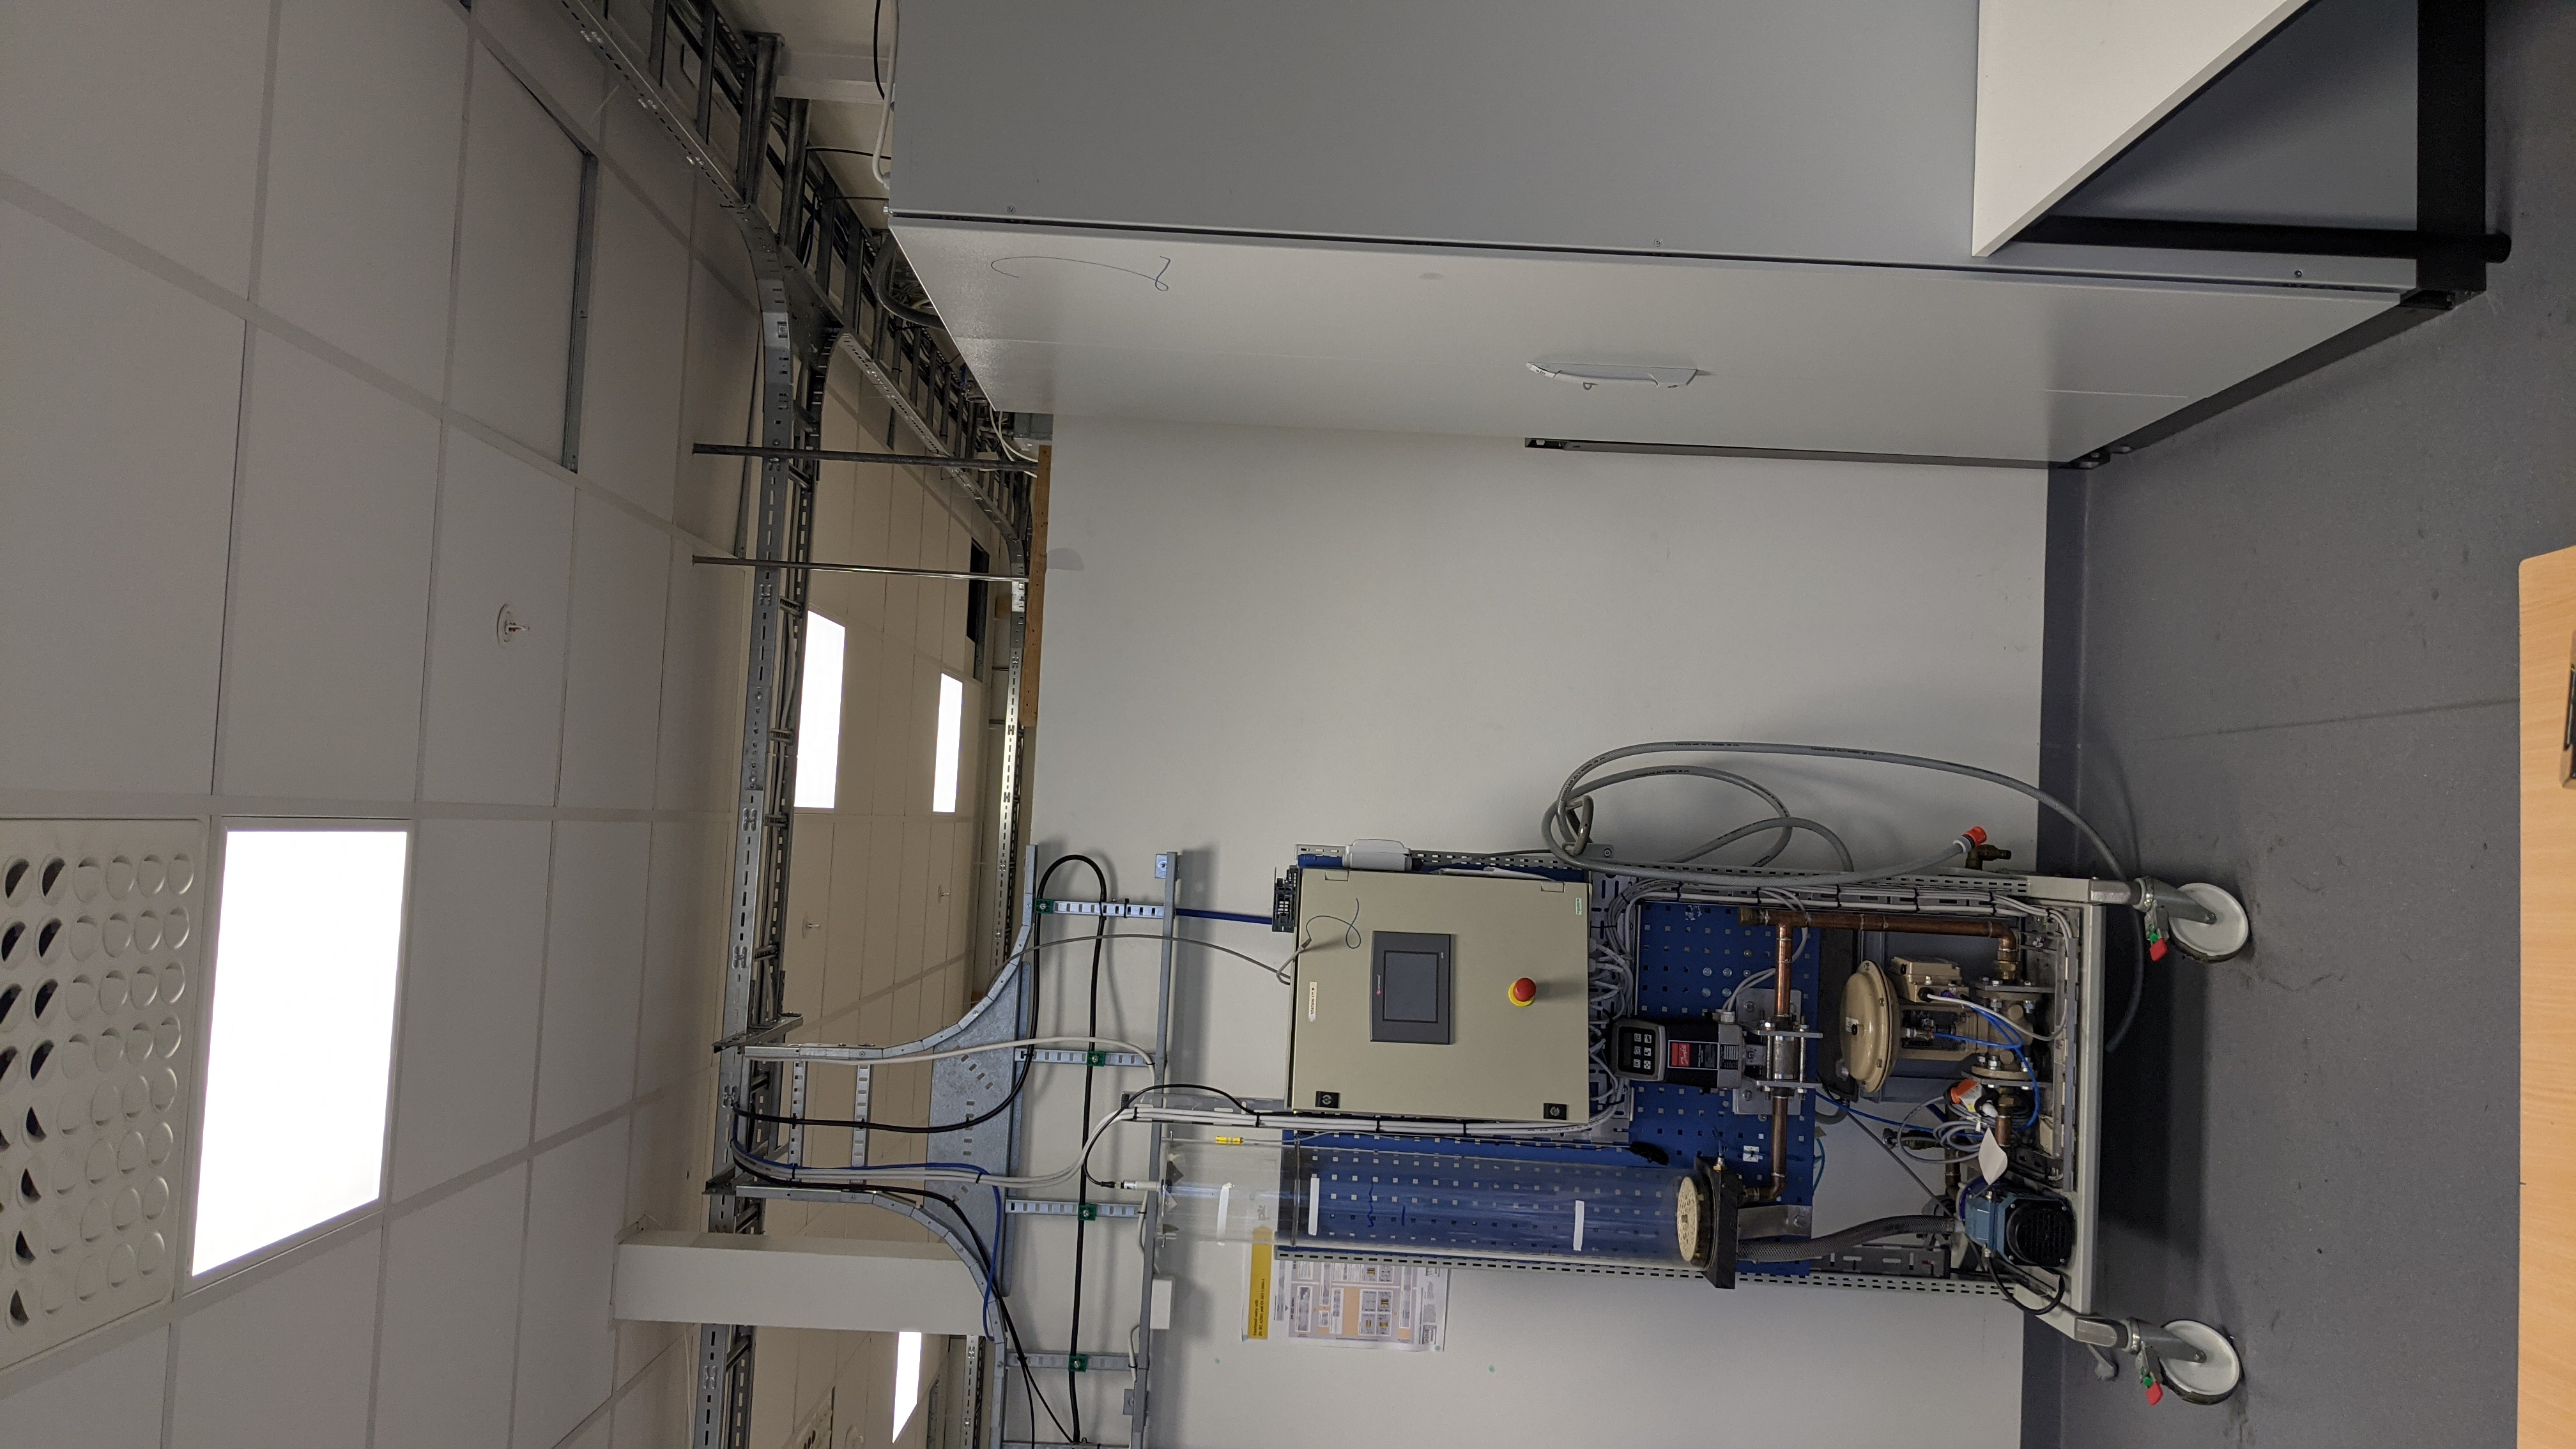
\includegraphics[width=10.5cm,angle=-90]{stasjon02x01.jpg}$$
\vskip 10pt 
\textbf{Introdusjon}

\vskip 5pt 
I dette oppdraget skal du koble det opp mot Stasjon2 med Siemens TIA portal og bruke dette programmet til å sjekke at tilkoblede signaler virker. om skjma ikke stemmer, må du tegne hvordan de faktisk er koblet. 

\vskip 5pt 
\href{https://rfka-my.sharepoint.com/:u:/g/personal/fred-olav_mosdal_skole_rogfk_no/EW7P-15mngBEih-uNAI5QJ0BVCWk1hocxIb7Rn_Sc1Df-g?e=hLlaex}{El-tegninger}

%$$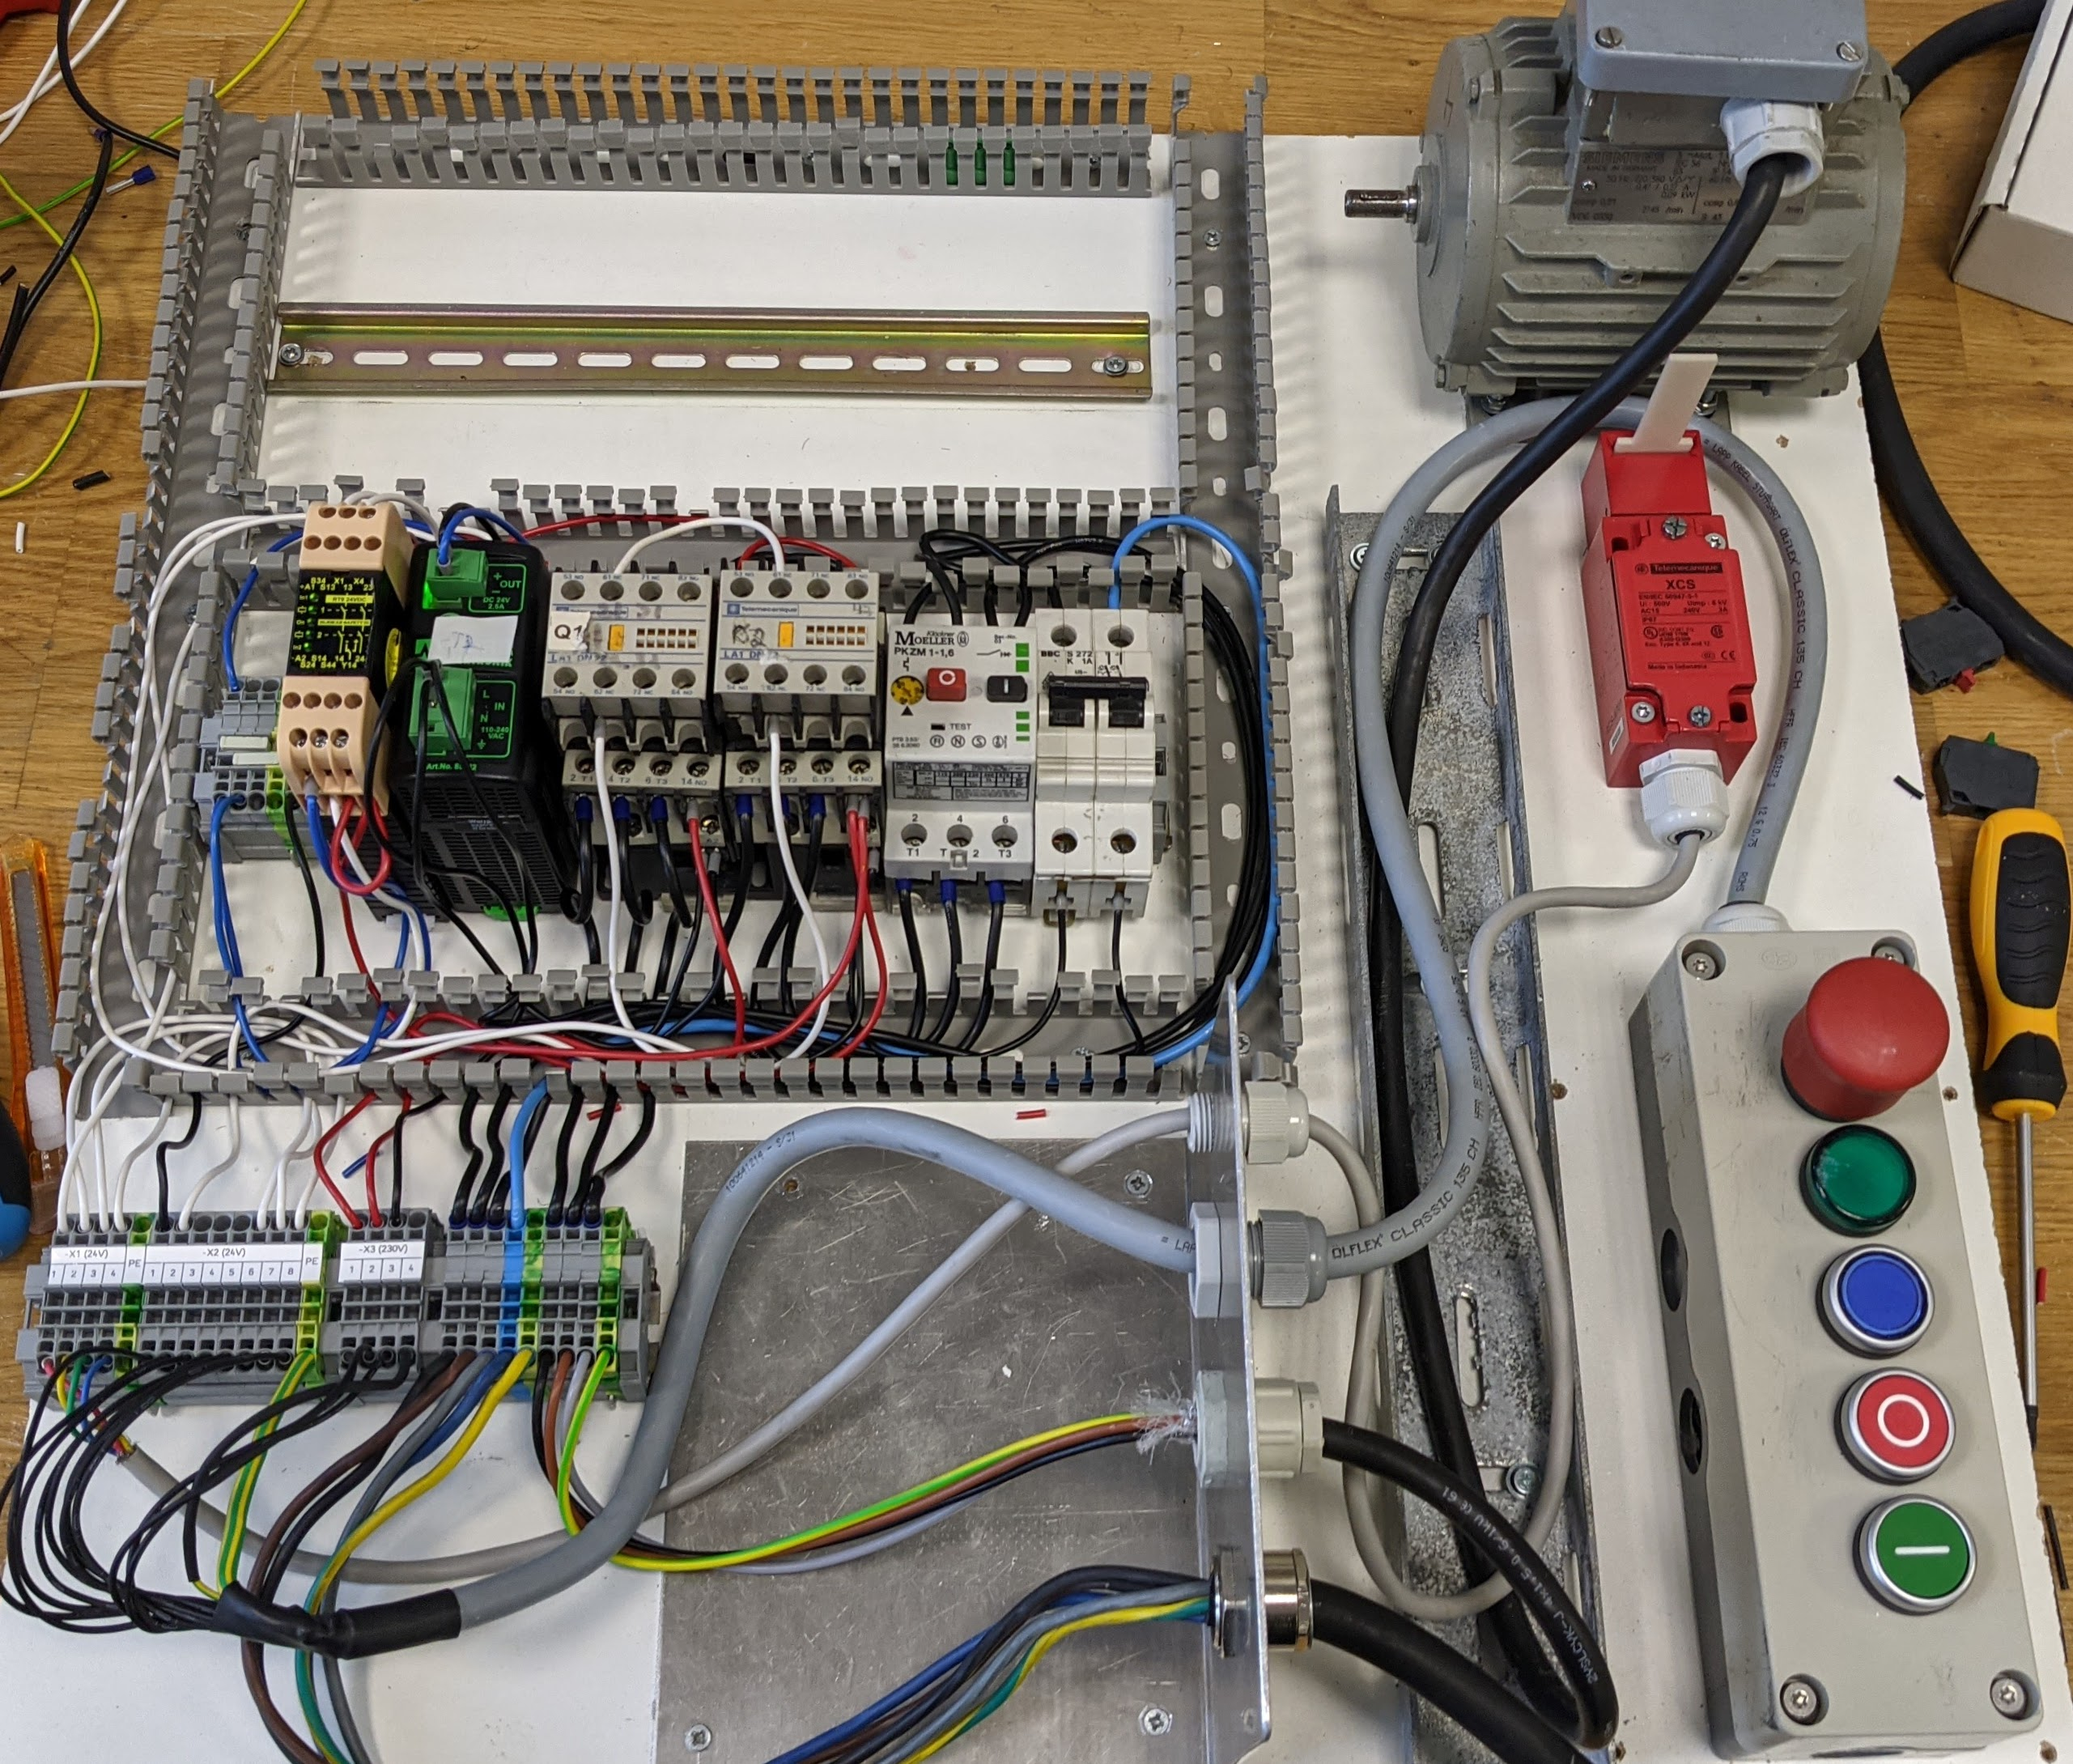
\includegraphics[width=13cm]{i04821x01.jpg}$$\\

\vskip 10pt 
\textbf{Teorioppgaver}

\vskip 5pt 
Sett eg inn i medfølgende el-tegniner og originalt skjema for skapet(finnesi papirform i skapet). Du skal være i stand til å følge signler og si hvilke som er korrekt tegnet og hvilke som ikke er det. 
\href{https://youtu.be/IqW5FCOWtC4}{Video tutorial Siemens TIA protal}

\vskip 10pt 
\textbf{Planlegging}


\vskip 10pt 
\textbf{Gjennomføring}

\vskip 10pt 
\textbf{Dokumentasjon}

Beskriv hvordan du planlegger, gjennomfører og dokumenterer denne jobben. 
















\underbar{file i04823}
\vfil \eject
%(END_QUESTION)





%(BEGIN_ANSWER)


%(END_ANSWER)





%(BEGIN_NOTES)


%INDEX% Arbeisdoppdrag, Styresystemer, Nivå 2, Stasjon02, IO-sjekk og dokumentasjon

%(END_NOTES)


